\documentclass{article}
\usepackage[utf8]{inputenc}
\usepackage[T1]{fontenc}
\usepackage[english]{babel}
\usepackage{enumitem}
\usepackage{amssymb}
\usepackage{amsmath}
\usepackage{color}
\usepackage[colorlinks,linkcolor=myorange, urlcolor=mygray, citecolor=mygreen, breaklinks, pagebackref]{hyperref}
\usepackage{graphicx}
\usepackage{caption}

\definecolor{mygray}{rgb}{0.7,0.7,0.7}
\definecolor{mygrey}{rgb}{0.5,0.5,0.5}
\definecolor{myorange}{rgb}{0.9,0.5,0}
\definecolor{mygreen}{rgb}{0.4,0.8,0}
\setcounter{totalnumber}{5}
\newenvironment{itemh}[0]{\begin{itemize}[font=\color{mygray} \small]}{\end{itemize}}
\newenvironment{itemH}[0]{\begin{itemize}[font=\color{mygray} \large]}{\end{itemize}}

\begin{document}
\title{Comparative Study about reasonning agents on RDF graphs using swarm computing}
\author{Baudouin Duthoit\\
Student number: 2540566
\and
Wouter Beek
\and
Stefan Schlobach
}
\maketitle

\abstract{
	RDF is a standard of W3C to enable computer and human to understand data, to give them sense.
	That is the Semantic Web.
	Data is stored in triples formed of a subject and a predicate and an object.
	Those triples themselves are on different computers well spread all over the web.
	More and more people are using the Semantic Web and so the online data is increasing a lot
	making the reasoning over the graph really complex and the more complex it is,
	the more we need efficient agents to increase performances.
	Our goal is to create agents that performs that reasoning base on the ants' behaviour
	and compare them to the bee agents we already have.
	We'll evaluate those agents empirically with tests on a sub-graph of the LOD.
	More information at \url{http://wouterblog.com/}.
}

\newpage

\tableofcontents

\newpage

\section{Introduction}
	\subsection{Presentation of the Semantic Web and RDF}
		%Introduction to RDF / Semantic Web
		\paragraph{} % Global presentation of RDF: The semantic web \& RDF
			Since its creation, the web see its data increasing exponentially.
			Those data are often unstructured and only human readable.
			Facing those two problems, scientists invented the semantic web to aggregate data
			and make it easy to access for humans and computers.\cite{Grigoris12}
			Those meta-data are structured in triples that are stored online in a lot of different places in RDF
			(Resource Description Framework).
			Each triple is made of a subject, a predicate and an object.
			A simple vision of the RDF graph could be to see it as a directed graph where a triple is a set of 2 nodes and an arc
			(predicate) from the subject to the object, thus we get a directed graph.
			However, the truth is a little bit more complex because predicates could also be nodes in some cases,
			and edges could be used several times.
			An RDF graph $G$ is a triple $\langle V, E, R \rangle$ consisting of a set of vertices $V$, a set of edges $E$,
			and an incidence function $R$ that maps edges onto pairs of vertices\footnote{
				Notice that an edge according to the latter definition is not an arc,
				because it is not a pair of vertices but mere associated with such a pair.
				This latter property allows $V$ and $E$ to have a non-empty intersection
			}.
			Also, there are several ways to store this data online.
		\paragraph{} % Data format
			The most common one is to put the data on a database and query it via SPARQL,
			which is language that look like SQL but for RDF.
			Then we can send a query and get back some results that are in that database.
			As for SQL, SPARQL could build some complicated queries.
			The other common way of getting data is directly get files containing RDF in it
			(RDF/XML, Turtle, Trig, N-Triples, N-Quads, JSON-LD, RDFa, ...).
			The last one is with deferenced data which is a mix of the two:
			it asks the server for data about a resource and get a file containing the data.
	\subsection{Related work}
		\paragraph{}
			The project repository is on GitHub\footnote{ \url{https://github.com/wouterbeek/DataHives}},
			it is mostly using SWI-Prolog\footnote{ Official website: \url{http://swi-prolog.org/}} language.
		\paragraph{} %Introduction to other work
			Last year, another bachelor student worked on a similar project.
			His goal was to get back information from a search using agents acting like bees (in JavaScript) \cite{Kroes13,Kroes13-2}.
			We used his code as inspiration for our own bee agents (that are programmed in prolog).
		\paragraph{} %Related work
			Our project is also linked to Kathrin Dentler, Christophe Gu\'eret and Stefan Schlobach's work
			about swarm computing\cite{Gueret10}.
			A swarm of other bachelor students is also working on Semantic web applications.
	\subsection{Hypothesis}
		\begin{center}
			\textit{
			In this project, we will compare the graphs induced by the bee walk,
			to the ones obtained by the random agents and also the one induced by the ant walk.
			We expect to have a high number of clusters with high betweenness centrality in the graph induced by the bee walk,
			and a pagerank-like graph for the random agents.
			The graphs induced by the walking behaviour of ants are expected to have a few components and a high connected one}
		\end{center}

	\subsection{Evaluation}
		\paragraph{}
			We will verify the hypothesis via different criteria.
			We'll make them work for a certain time and then compute the betweenness centrality and the clustering coefficient.
			We will also vary the number of agents to see if there are some big variations or not (saturation ?).
			Those two methods will be used to compare 3 kinds of agents:
		\begin{itemh}
			\item Random (basic)
			\item Bee (translated from JavaScript)
			\item Ant (Implemented from scratch)
		\end{itemh}

\newpage
\section{Approach}
	\paragraph{}
		In this section, we'll talk about how did we choose to solve the problem that was stated in the introduction.
		First, we'll give definitions that we'll use latter where we'll present what an agent is.
	\subsection{Definitions}
		\paragraph{}
			Most of the definitions are from ``Graph Theory and Complex Networks''\cite{Steen10}
		\paragraph{Path}
			Consider a graph $G$.
			A $\langle v_0 , v_k\rangle-walk$ in $G$ is an alternating sequence $\langle v_0 , e_1 , v_1 , e_2 \dots
			v_{k-1} , e_k , v_k \rangle$ of vertices
			and edges from $G$ with $e_i : \langle v_{i-1},v_i \rangle$.
			In a closed walk, $v_0 = v_k$ .
			A trail is a walk in which all edges are distinct; a path is a trail in which also all vertices are distinct.
			A cycle is a closed trail in which all vertices except $v_0$ and $v_k$ are distinct.
		\paragraph{Connected}
			Two distinct vertices $u$ and $v$ in graph $G$ are connected if there exists a $\langle u, v \rangle - path$ in $G$.
			$G$ is connected if all pairs of distinct vertices are connected.
			A digraph (directed graph) $D$ is strongly connected if there exists
			a directed path between every pair of distinct vertices from $D$.
			A digraph is weakly connected if its underlying graph is connected.
		\paragraph{Component}
			A sub-graph $H$ of $G$ is called a component of $G$ if $H$ is connected
			and is not contained in a connected sub-graph of$G$with more vertices or edges.
			The number of components of $G$ is denoted as $\omega(G)$
		\paragraph{Clustering coefficient}
			In the book of Maarten Van Steen it is written :
			``We can express the existence of communities by means of a clustering coefficient''\cite{Steen10}
			That gives the semantic meaning of this mathematical calculation below,
			knowing that $n_v$ is the number of neighbours of $v$
			and $m_v$ is the number of edges in the sub-graph induced by $N(v)$.
		\begin{align*}
			cc(v) = \begin{cases}
				m_v/ \binom{n_v}{2} = \frac{2*m_v}{n_v(n_v-1)} & \text{if } \delta(v) \ge 1 \\
				undefined & otherwise
			\end{cases}
		\end{align*}
		\paragraph{Betweenness centrality}
			Let $G$ be a simple, (strongly) connected graph.
			Let $S(x, y)$ be the set of the shortest paths between two vertices $x, y \in V(G)$,
			and $S(x, u, y) \subseteq S(x, y)$ the ones that pass through vertex $u \in V (G)$.
			The betweenness centrality $c_B (u)$ of vertex $u$ is defined as
		\begin{align*}
			c_B (u) = \sum \frac{|S(x,u,y)|}{|S(x,y)|}
		\end{align*}
		\paragraph{Density}
			Consider a simple, undirected graph $G$ with $n$ vertices and $m$ edges.
			The network density $\rho(G)$ of $G$ is defined as $\frac{m}{\binom{2}{n}}$ .
	\subsection{An agent?}
		\paragraph{}
			Our work on the agents is based on this book \cite{Engelbrecht05}.
			An agent is a small program computed to do intelligence on his own.
			In our case an agent would do research and/or entailment,
			it is also part of a population.
			Its behaviour is often based on an animal, we will use the bees and the ants for our study.
		\paragraph{}
			A population is a set of agents that work together to aim or reach a certain goal.
			Even if the goal of this paper is to find the difference between the graphs generated by different agents,
			the population aims to get information from entailments or to search for information.
		\paragraph{}
			All the agents are implemented in the same way.
			They follow a cycle of events and repeat that cycle.
			The cycle to follow is:
		\begin{center}
			Navigate / Act / Communicate / Evaluate
		\end{center}
		\paragraph{}
			Navigation is the function that decide \textbf{where} the agent should go, depending on where it is already.
			In facts, this predicate pick a proposition between all the possibilities,
			those possibilities could be, for example, all nodes that are neighbours to the one we are on.
			The kind of agents define what are the several possibilities.
			The graph containing all the neighbours is called the ego-graph of the chosen node,
			we assume it contains all the incoming and out going neighbours.
			Unfortunately, those nodes could be literals and then we could get stuck on it because literals are linked to nothing.
			To avoid that, we have a backtrack function that keeps in mind the last position we were on.
		\paragraph{}
			Acting is where the agent do what it is meant for when it is on his own.
			In a clearer way it means that in this step the agent should work on the node it is on.
			This step is a selfish one where the other agents don't matter at all.
			The main action is only the deductive action of entailment.
			The rules for that can be found on the W3C web page\footnote{
				\url{http://www.w3.org/TR/2014/REC-rdf11-mt-20140225/\#rdfs-entailment
			}}.
			We apply all of them to get some more information.
			Because all agents will have the same action, we decide to describe it here.
		\paragraph{}
			Communication is the main point of those agents.
			We try different kind of communication to see whether one is more efficient than the other
			and then compare the different kind of agents.
		\paragraph{}
			The evaluation part decides whether an agent deserve to continue his job or not.
			If it is judged inefficient then we throw it away using the exit function given at the creation of the agent.
			It's here where the fitness function should act.
	\subsection{Random Agent}
		\subsubsection{Navigate}
			\paragraph{}
				The random agent is implemented to go randomly.
				It is initialized on a set of available URI where to begin.
				This set of available URI could be all the possible random URI of dbpedia reachable by the random jump function,
				as it could be a hand written list of URI's in the code.
				Then it goes, following ``links''.
				Those links are the predicates between 2 nodes of the Linked Open Data (LOD).
				After his walk, his path is a connected graph of every places he has been.
		\subsubsection{Communicate}
			\paragraph{}
				The communication is not implemented to stick to a really basic agent attitude that will serve as reference for efficiency.
		\subsubsection{Evaluate}
			\paragraph{}
				The evaluation function is not set for this kind of agent that keep going whatever happens.
		\subsubsection{At exit}
			\paragraph{}
				This predicate is not used because it is really bound to the evaluation of the agent (previous step) that we discarded.
	\subsection{Ant Agent}
		\subsubsection{Navigate}
			\paragraph{}
				The ant navigation is based on randomness but a weighted one.
				Like an ordinary ant, our agent has to pick a path, depending on the pheromones left on it.
				On the virtual web of the LOD cloud, the pheromones are coefficients left on edges from one node to the another.
				If another ant went here before, the path get more value, and has more chance to be choosen.
		\subsubsection{Communicate}
			\paragraph{}
				As said above, an ant leave pheromones wisely.
				The insect is looking for food (= information) outside (= on the LOD cloud or on a sub-graph of it).
				When it has found something, it goes back to the anthill and leave pheromones on its way back as well.
				The main idea here is to up value a path which leads to food and devalue one that leads nowhere (ie dead-end path).
				To represent this virtually here was our main ideas with $c \in \mathbb{N}$:
			\begin{itemh}
			\item Devalue dead end path, using SPARQL queries to go back and degrade the weight of the path of $c$
			\item Adding $c$ to all the travelled path for each information deduced
			\item Adding the agent's current fitness to the current edge
			\end{itemh}
			\paragraph{}
				All those ideas needs to be tried and evaluated to see which one is the more efficient and if we could cross them.
		\subsubsection{Evaluate}
			\paragraph{}
				The evaluation is where the fitness function is used.
				For ants, the fitness function is quantitative,
				counting the number of triples discovered via deduction and dividing it by the number of steps taken.
				If that number is bigger than 0.5, the agent can live, otherwise it dies launching the exit function.
		\subsubsection{At exit}
			\paragraph{}
				When the time comes for an agent to kill himself, it is decided that it must launch another agent to replace him.
				And so, the agent launch another agent that will work to get more information that the previous one if possible.
			\paragraph{}
				For the test we've made on ant agents,
				we decided to let this function empty to let the agent get killed after a certain number of steps,
				otherwise, the evaluation would have never stop, creating agents after agents.
				Another asset we could obtain doing so is that we get a maximum number of steps that we could state from the beginning
				(it enable the possibility of choosing a graph's size).
				This infinite loop of agent is on purpose because we want this to work without any end.
	\subsection{Bee Agent}
		\subsubsection{Navigate}
			\paragraph{}
				A bee navigates randomly, whatever her role is.
				A scout jumps from one place to another one (that could be at the opposite side of the whole graph).
				However, a forager navigates like a random agent: following links.
				The scouts are wandering around to try to find information.
				When one succeed, it tells some others (called forager) to come and grab the ``pollen'' it has found.
		\subsubsection{Communicate}
			\paragraph{}
				Here the communication is really simple.
				It directly contacts the other agent to tell them something:
				the information is not sustainable, it is not stored somewhere.
				The information send is used instantly (it makes it more easy to set up).
			\paragraph{}
				In our case, the ``communication'' is not really a communication between agents:
				it creates the agents that should receive the message to go work next to the discovered node.
		\subsubsection{Evaluate}
			\paragraph{}
				The evaluation is based on the same criteria of the one for the ants but here it triggers an action.
				If the fitness is big enough we send some foragers helping the scout, but if it is too low \dots the agent get killed.
		\subsubsection{At exit}
			\paragraph{}
				At the end of the thread it also asks for another agent to replace himself and keep sustainability in getting information.
				As for the ants, this function is left empty for the evaluation.

\section{Implementation}
	\subsection{Developing tools}
		\subsubsection{Prolog}
			Prolog is a general purpose logic programming language associated with artificial intelligence and computational linguistics.
			Prolog has its roots in first-order logic, a formal logic, and unlike many other programming languages,
			Prolog is declarative: the program logic is expressed in terms of relations, represented as facts and rules.
			A computation is initiated by running a query over these relations.
		\subsubsection{Emacs}
			Emacs for Prolog has been used a lot.
			The asset of this text editor was to put a semantic text colouration
			or just simply show within the code if a specific module was necessary or not.
			It was also used by the debugger, with the same text colouration (useful if you don't want to get lost).
		\subsubsection{\LaTeX}
			\LaTeX \hspace{1mm}has been used to write this report in a scientific way.
	\subsection{Debug tool}
		\subsubsection{Web UI}
			\paragraph{}
				This section will present what features already implemented in the project are in use.
				What we have access in this interface to the graph the agents have been crawling.
				It is a way to visualize the graph that as been created by the agents.
				It has also been used as a debug tool: if the graph contains only one node with one edge where the agent passed 200 times,
				that means that there is something fishy about the navigation strategy.
				Another good example was with the bee algorithm, where a lot of nodes where alone, with no neighbours.
				In that case, it meant that the communication or the evaluation was wrong (either calling forager or the fitness were bad).
			\begin{figure}[!h]
				\hspace{-2cm}
				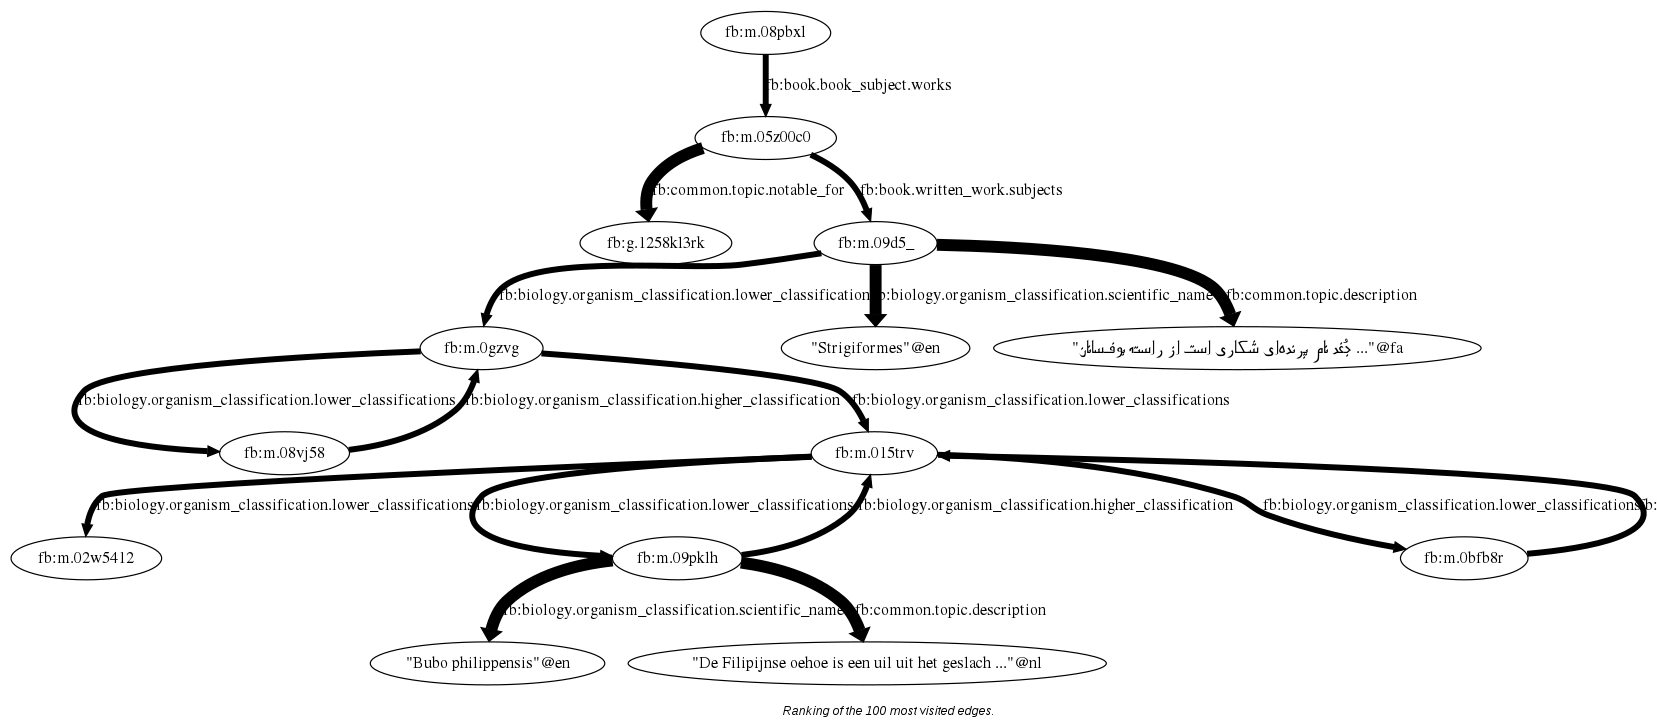
\includegraphics[width=1.4\textwidth]{../dh_graph}
				\captionof{figure}{Sketch of the graph}
			\end{figure}
			\paragraph{}
				This Web interface also enable show a table containing all the agents working at the moment
				on the graph with their status (running / exited / \dots).
				If one of the agent crash, it shows up and the reason why.
		\subsubsection{Debugger}
			\paragraph{}
				The debugger was one of the main debug tool used.
				It enables the developer to get step by step into the code.
				It has been used to find how does the code works, because the project was already quite big when I started working on it,
				and also why it didn't work when some new functions were implemented.

\section{Evaluation}
%	\subsection{Quantitative Evaluation}
%		\paragraph{}
%			First, we want to compare the agents over the number of deductions over the time they are running.
%			It is something simple to count and objective, but it may be not relevant (if we look at the semantic part).
%			To be more accurate, we have used 100 agents of each category, and run them for a certain time.
%			Of course, it is running on the same machine to have the same environment as much as possible.
%		\begin{center}
%			\textit{Place for a future graph, comparing agents x = time, y = deductions}
%		\end{center}
%		\paragraph{}
%			Description of the graph and deductions
	\subsection{Find the right size graph}
		\paragraph{}
			Several options were open for the agents' evaluation.
			First of all, testing the agents on the LOD cloud and then working on the results.
			This try gave us trouble because finding a random triple for the ``random\_jump'' used by the scout agent
			on the LOD cloud is really slow, because the LOD cloud is really big.
			We need to know all the available triples at the time of the request before choosing one randomly in that list,
			if a server goes down between 2 steps (between 2 random jumps), we have to refresh that list,
			thus, the tests about the bee agents are not feasible (using a random triple for each cycle).
			A first solution was to find a random triple from dbpedia using a dictionary.
			A dictionary containing 40 000 words, we tried to get the equivalent resource
			(if it didn't exist, we would have picked another one),
			then we choose a random node linked to that one (multiplying by 100 the diversity) we obtain a ``random'' node from dbpedia
			(which some times get down as well).
			On the other hand, taking a dataset from the data laundry was an interesting solution
			(we are sure to get a fix data set for all the tests, and the dataset is clean of mistakes).
			We tried a data set of size 1,001 triples, another of 1,003,529 triples and the biggest one of around 10,000,000 triples.
			The first one was too small to execute relevant tests (each time all the graph was totally crawled several times).
			The biggest one was the second try but gave too few results due to the huge size of it.
			The last one gave the more encouraging results with a runtime of 30min, for all the agents to fulfil their tasks
			(a total of about 10 000 steps for all the agents).
	\subsection{Graph figures comparison}
		\paragraph{}
			We formulate in the hypothesis that the crawled graph must differ between every kind of agents.
			To prove this, we have been using Gephi\footnote{
				Here is the software website \url{https://gephi.github.io/}
			} to dig out some figures from our graphs.
			The more representative figures were the betweenness centrality and the number of components.
			The work on the graph is based on the content of the class ``Networks ans graphs'' followed this year,
			which was referenced on this book \cite{Steen10}.\\
		\newline
			To be more clear about the test, here is the followed protocol:
			\begin{itemH}
				\item Changing in the code the number of steps before death for an agent
				(could be implemented later in the evaluation module).
				\item Server initialization
				\begin{itemh}
					\item start the prolog application ($swipl\hspace{1mm} run.pl$ in the console)
					\item load the test module
					\item run $evaluation(X,Y).$ where X is the type of agent and Y is the number of it.
				\end{itemh}
				\item Check the agents runtime/state on the web UI
				\item When all the agents are done, export the graph of what they have crawled
				\item Reset/shut down the server
			\end{itemH}
		\paragraph{Test with 1 scout and 1000 steps}
			The graph we got from such a configuration contains 1209 nodes and 998 edges.
			The plot below is showing the nodes where the betweenness centrality is higher than 0
			(1120 nodes have a null value for betweenness centrality, they are not represented here for more readability).
			A null betweenness centrality means that no shortest path go through that specific node,
			in our case, it concerns all the nodes on the edge of the graph which explain such a high value
			(the $random_jump$ predicate creates a lot of those nodes because it creates a
			lot of components where the scout may not call the foragers).
			The clustering coefficient is almost always equal to zero.
			It means that there are no triangles in the graph.
			A surprising fact is the number of components: the scout is supposed to jump from places to places 1000 times
			but create only 211 components.
			The only cases where a component is not created is if a scout is jumping on a node that already exists on one hand,
			or on the other hand, when a forager meets a node that have been visited by another agent before
			(then the 2 components become one).
		\begin{figure}[!h]\hspace{2cm}
			\includegraphics[height=6cm]{dh_betweenness_centrality_1_scout}
			\captionof{figure}{Betweenness centrality figures for 1 scout agent}
		\end{figure}
		\paragraph{Test with 100 scouts and 10 steps for each}
			To see if the number of agents is a significant factor, we executed a test with 100 scouts that only jump 10 times.
			The total number of steps stays the same and because the 100 agents are jumping randomly over the graph,
			we could expect the same results as the one we got with one agent crawling over 1000 nodes
			(and that's what we got).
			The only difference is in the speed of the evaluation because 100 agents are easier to execute in parallel than one,
			thus we get results faster.
			The number of components is 196, quite close to 211.
			So the number of agents is not a changing the behaviour of the population, in case of bee agents.
		\begin{figure}[!h]\hspace{2cm}
			\includegraphics[height=6cm]{dh_betweenness_centrality_100_scouts}
			\captionof{figure}{Betweenness centrality figures for 100 scout agents}
		\end{figure}
		\paragraph{Test with 1 random agent and 1500 steps}
			Here, we expect to find a low density graph, and that's what we have: $\rho = 0,004$ (a complete graph density is equal to 1).
			The graph below show that over 881 nodes, some are on more than 30\% of all the shortest paths between every nodes.
			That's much more than we got on the scouts plot about betweenness centrality.
			Also, we can notice the small amount of edge nodes (106 over 881).
			At last but not least, the density is null.
		\begin{figure}[!h]\hspace{2cm}
			\includegraphics[height=6cm]{dh_betweenness_centrality_1_random_agent}
			\captionof{figure}{Betweenness centrality figures for 1 random agent}
		\end{figure}
		\paragraph{Test with 100 random agents and 150 steps each}
			Here, we have done 15 000 steps in total and we have only one component.
			That means that the 100 agents crossed each other path to form one component in the end
			(because they started from random nodes).
			Also, the number of steps/agents does not matter because the results are quite the same with only 1 agent.
		\begin{figure}[!h]\hspace{2cm}
			\includegraphics[height=6cm]{dh_betweenness_centrality_100_random_agent}
			\captionof{figure}{Betweenness centrality figures for 100 random agents}
		\end{figure}
		\paragraph{Test with 1 ant agent and 1500 steps}
			The ant agent show some surprising results.
			First of all, some nodes have a betweenness centrality of 0.5,
			that means that more than a half a the shortest path go through them, that's a lot.
			We could imagine that those nodes are linked to a lot of other nodes and thus enable such quick path between 2 nodes.
			However, we should have found such a node in the previous try as well.
			We could suppose that the ant agent as created a main path and then get stuck on it because it gain some importance.
			The density is of 0.005,
			so we could may be deduce that the component is more connected than the graph induced by the random agent.
		\begin{figure}[!h]\hspace{2cm}
			\includegraphics[height=6cm]{dh_betweenness_centrality_1_ant}
			\captionof{figure}{Betweenness centrality figures for 1 ant agent}
		\end{figure}
		\paragraph{Test with 100 ant agents and 30 steps each}
			As we already saw, the number of agents is not changing that much the results.
			We can also say that the betweenness centrality of 0,5 was not fortunate because we have it again,
			of course, it could be a bias induced by the dataset,
			but it would have showed up for the previous tests with different agents as well.
			The only figure that is changing is the density value (equal to 0.002), but this may be due to the bigger size of the graph.
		\begin{figure}[!h]\hspace{2cm}
			\includegraphics[height=6cm]{dh_betweenness_centrality_100_ants}
			\captionof{figure}{Betweenness centrality figures for 100 ant agents}
		\end{figure}
		
\section{Reflection}
	\paragraph{}
		This section introduce what problems have been faced and did we react to them.
		It is showing some hidden problems that slowed the project or some other more obvious that we solved (or tried to).
	\subsection{Dead end paths}
		\paragraph{}
			The LOD is a big graph on which it is really easy to get lost.
			Especially in some dead end path, because the graph is directed, going back is not easy.
			In fact, the agent only memorize the last step he has done (to optimize memory usage),
			because the graph is directed, the links between the nodes are one way only and don't appear on the last link they've been on.
			We have a backtrack function in case of which we would have arrived on a literal (special case),
			But this backtrack function is only limited to go one step backward.
			Storing the whole path would be memory inefficient.
		\paragraph{}
			To solve this, we start an action when an agent detect when it is in a dead end path (when it can't go anywhere).
			This specific action is quite simple, it start from the node where the agent got stuck and devalue the path to it.
			To know the path, we just crawl the cache starting from the “blocking node”
			and see if there are other possibilities that the one we come from.
			If yes, it means that the node we just arrived on is the end of the dead end path.
			If no, we just repeat the previous step to find that node which show the end of the path.
			Also, we kill the agent and create a new one instead that will crawl from another place.
	\subsection{Denied access}
		\paragraph{}
			The LOD contains some restricted area we the agents cannot go.
			When an agent meet such a place, it just go backward of one step.
			Sometimes, it is also because the server where we try to grab information from is down.
			Some of them, like dbpedia have a live version of it which is sometime replacing the other one,
			so we just try all different access point we know to get data from.
	\subsection{Difficult tests} %Be more accurate
		\paragraph{}
			At the beginning, the ant agents used to go really often in dead end alley
			or find information that did not follow one of the standardized grammars for RDF serialization and crashed,
			and after a crash, we launch another ant from another random place on he graph.
			That made the testing quite complicated, because the data we got from the whole population was too diverse to be relevant.
			The agents were to often far apart from each other (and the communication was quite useless then).
	\subsection{Keep as minimum the communication between threads} %
		\paragraph{}
			Even if we want the agents to communicate with each other, it is better if their communication remain light,
			otherwise, they spend too much time waiting for each other and the efficiency becomes bad.
			For example, the system we work on don't have a kind of mother-ship that give orders.
			Each agent is working on his own and has is own independent functions.
			Also, the agents communicate with each other only is they are told to.
			Ants are leaving their communication on the trail and thus don't really use a communication system.
			Bees are creating forager on the spot rather than calling some that would have been working somewhere else.
			So in the end, the thread communication is not used for our system.
		\paragraph{}
			A necessary communication that has been established between threads is a message system to get information about the thread,
			like the number of steps taken.
			This system is to take information about the population and is also as light as possible to don't get the mother-ship problem.

\newpage
\section{Conclusion}
	\subsection{Results}
		\paragraph{}
			After several tests over the populations of agents, we lead on conclusions.
			First of all, about the population size.
		\paragraph{}
			Actually it seems that the number of agents is not a significant factor to evaluate a population
			because we obtained figures that were quite alike independent in the number of agents.
		\paragraph{}
			The betweenness centrality value and its repartition over the whole group of nodes for each graph
			shows a clear difference between the graph we obtained from the different kind of agents.
			Also, the graph induced by the bee walk showed a high amount of components rather than clusters,
			as stated in the hypothesis.
		\paragraph{}
			The pagerank like behaviour expected of the random agent is not obvious,
			even if the betweenness centrality shows an exponential curve about the importance of the agents on a shortest path perspective,
			we don't have the tools to know whether those nodes are important or not from another perspective
			(a subjective one, for example).
		\paragraph{}
			The ant agents showed an interesting structure of a graph with only one component and a betweenness centrality of
			0.5 for some special nodes.
			For the next experimentations, we could try to visualise such a graph.
	\subsection{Thanks}
		\paragraph{}
			I would like to thank the VU university from Amsterdam to makes me able to study here for this year.
			I also want to thank Stefan for accepting me to do my Bachelor thesis with him
			and I especially thank Wouter for his help during all this project.

\newpage
\bibliographystyle{plain}
\bibliography{bibliography}
\addcontentsline{toc}{section}{Bibliography}
\end{document}
